\section{Magnetic sectors with holes of positive radius}
\label{sec:sectors}

We first determine the sector ratio on a fixed domain whose holes have
positive radius. The holes remove every source of the connection, but
retain its periods. The height limits of Section~\ref{sec:heights} then
determine the cost of these periods through a variational energy.
This result will be used before any hole radius is allowed to shrink.

\subsection{The sector theorem and its upper bound}

Let \(U\) be a bounded connected polygonal domain with a simple outer
boundary and finitely many simple polygonal holes. All sides are parallel
to the coordinate axes and have dyadic endpoints. The closures of the
holes are mutually disjoint and lie strictly inside the outer boundary;
every boundary segment has positive length. In particular, \(U\) is
Lipschitz and has no point contacts.
The graph \(\mathcal G_n(U)\) is the nearest-neighbor discretization at mesh
\(n^{-1}\), with free boundary and coherent array rounding as in
Definition~\ref{heights:geometry}.

Fix integral periods around the holes, in units of \(2\pi\), and a smooth
closed one-form \(dv_0\) with these periods, defined on a neighborhood
of \(\overline U\). Here \(v_0\) denotes a multivalued primitive:
its local branches differ by constants and its differential is
single-valued. A sum of integer multiples of angle functions, with centers
in the holes, provides such a form. Let \(\alpha_n\) be an integral
connection on \(\mathcal G_n(U)\), flat away from the holes, with the prescribed
periods. Its sector ratio is denoted by \(F_{U,n}^s\).
Changing \(\alpha_n\) by an integral gradient leaves this ratio unchanged.

\begin{theorem}[Sector cost at fixed geometry]\label{sectors:positive-radius}
For the domain and periods just specified, at \(b=b_c\) and
\(a=8\pi\),
\begin{equation}
 \lim_{n\to\infty}F_{U,n}^s
   =\exp\{-\mathcal M(U)/(2a)\},
 \qquad
 \mathcal M(U)=\inf_{g\in H^1(U)}
                    \int_U|dv_0+dg|^2 .
 \tag{3}\label{eq:source-3}
\end{equation}
The limit holds along every admissible mesh-rounding sequence.
The variational energy depends only on the periods.
\end{theorem}

The upper bound extends the divergence-free real-tilt argument of
\cite[proof of Proposition~2.6]{C} to this fixed multiply connected
domain. For the lower bound we add strong, spatially distributed
confinement. Its separated zero-pin interactions vanish, which controls
the restoration loss after averaging over guard data. We can then slit
every hole, apply the single-valued height limit on the resulting pieces,
and restore the cuts.

\begin{proof}[Proof of the upper bound]\label{sectors:upper}
Choose a smooth stream function \(\psi\) constant in a neighborhood of
each boundary component, allowing different constants on different
components, and put \(w=\nabla^\perp\psi\). Thus \(w\) vanishes near the
boundary. Sample \(\psi\) on the faces of the height graph and take
oriented differences across its edges. This gives an exactly
divergence-free edge flow \(w_n\), supported away from the boundary,
whose coefficients are \(n^{-1}w\) to first order.
The form \(dv_0\) and \(\alpha_n\), integrated along lattice edges, have
the same cycle periods. Their difference is therefore a real gradient.
Consequently
\[
 D_n'=\sum_e w_{n,e}(\nabla_e h+\alpha_{n,e})
     =\sum_e w_{n,e}\alpha_{n,e}
       \longrightarrow \int_U w\cdot dv_0
\]
is deterministic.

Insert \(e^{D_n'}\) into the sector numerator. Partition \(U\) into
dyadic squares of side \(d\), with \(d\) fixed and aligned with the
boundary, and cut all edges between distinct squares.
In applying Lemma~\ref{heights:cut-comparison}, retain an independent
Bessel increment on each cut edge and place that edge's tilt on this
increment. Restoring the edge identifies the increment with the affine
height difference, so the statistic has not changed. The normalized
tilted sector sum is bounded above by the resulting product of
centered Laplace transforms. On each square the connection is an
integral gradient and disappears by reindexing heights. Since the tilt
is on the affine differences, this reindexing introduces no scalar
tilt factor.

Here is the limiting bound on that product. On the internal edges of
each square replace the coefficients of \(w_n\) by \(n^{-1}\) times
one constant vector sampled there, and set the replacement to zero on
cut edges. For fixed \(d\), the sum of squared errors on cut edges is
\(O_d(n^{-1})\): there are \(O_d(n)\) such edges and every coefficient is
\(O(n^{-1})\). The remaining squared error has a limsup tending to zero
as \(d\downarrow0\), by smoothness of \(w\).
The free-square Laplace limit in Theorem~\ref{heights:free-input}
applies to the constant-vector tests. Their total limiting log
transform is \(a/2\) times the corresponding Riemann sum for
\(\int_U|w|^2\).

For completeness, the errors can be kept inside the transforms.
Apply H\"older's inequality with exponent \(p>1\) to the constant-vector
part. Bound the transform of the error, at the conjugate exponent,
by freeing all Bessel increments. For every fixed tilt multiple,
\[
 \log\E\exp\!\left\{\sum_e r_e J_e\right\}
 \le C\sum_e r_e^2
\]
when the \(J_e\) are independent increments of law \(p_{b_c}\) in
height units and the \(r_e\) are uniformly bounded.
This follows from
\(\E e^{tJ_e}=\exp\{b_c(\cosh(2\pi t)-1)\}\).
First let \(n\to\infty\), then \(d\downarrow0\), and finally
\(p\downarrow1\). We obtain
\begin{equation}
 \limsup_{n\to\infty}\log F_{U,n}^s
 \le -\int_Uw\cdot dv_0+\frac a2\int_U|w|^2.
 \label{sectors:dual-bound}
\end{equation}

The fields \(w\) just used are dense in the orthogonal complement of
gradients in \(L^2(U;\R^2)\). Indeed, extend a field in that complement
by zero outside \(U\). Its distributional divergence vanishes, so in
a larger simply connected box it has an \(H^1\) stream function.
This function is constant on every complementary component of \(U\).
Subtract a smooth function having the same constants near these
components. The remainder has zero trace on \(\partial U\), and
\(H^1_0(U)\) approximation now proves the density assertion.
The gradient space is closed by the Poincar\'e inequality modulo
constants. If \(P\) is the orthogonal projection onto its complement,
then \(\mathcal M(U)=\|P\,dv_0\|_2^2\).
Optimizing Equation~\eqref{sectors:dual-bound} over the dense class,
with optimizer \(a^{-1}P\,dv_0\), gives the required upper bound.
\end{proof}

\subsection{Confinement suppresses separated pin interactions}

We next add one quadratic observation for each small cell. Although
each observation has coefficient one, their number grows as the cell
size decreases. This gives the lower-bound construction its spatial
localization.

Fix one of the polygonal geometries of
Definition~\ref{heights:geometry} whose rectangular pieces have
dyadic coordinates, possibly with finitely many components or cuts.
Partition it into dyadic squares \(Q\) of side
\(d\), aligning all boundaries and cuts, and write
\[
 u_Q=\frac1{|Q|}\int_Q u,\qquad
 \mathcal T_d(u)=a^{-1}\int|\nabla u|^2+\sum_Q u_Q^2 .
\]
The lattice observation on \(Q\) is the average over its rounded array
of vertices. Its penalty is one half of the square of that average.
These observations control the constant on every component.
For two positively separated unions of positive-area boxes \(H,p\)
with dyadic coordinates,
let \(D_{n,d}(H,p)\) be the centered absolute-zero pin interaction of
Theorem~\ref{heights:pin-input} for this law.

\begin{lemma}[Localization under cell observations]
\label{sectors:localization}
For every fixed dyadic mixed geometry and fixed dyadic pin regions
\(H,p\) as above,
\begin{equation}
 \lim_{d\downarrow0}\limsup_{n\to\infty}D_{n,d}(H,p)=0 .
 \tag{4}\label{eq:source-4}
\end{equation}
Here \(d\) runs through dyadic values aligned with every fixed
geometric division. The mesh limit is taken at each fixed \(d\).
\end{lemma}

\begin{proof}
At each fixed \(d\), Theorem~\ref{heights:pin-input} identifies the
limit with the Gaussian determinant in Equation~\eqref{eq:source-1}.
We prove that this determinant tends to one.
Equip the component \(H^1\) spaces with the norm
\(\|u\|_d^2=\mathcal T_d(u)\), and write
\[
 V_Q=\{u:u=0\text{ on }Q\}^{\perp_{\mathcal T_d}},\qquad
 C_d=\Pi_H|_{V_p},
\]
where \(\Pi_H\) is orthogonal projection onto \(V_H\).
The letter \(Q\) in this definition can denote a pin region;
the observation cells remain the squares in the sum defining
\(\mathcal T_d\).

Rescale space by \(d^{-1}\). The observation cells are now unit
squares. In dimension two the gradient energy is unchanged by this
rescaling, and cell Poincar\'e gives, with constants independent of \(d\),
\begin{equation}
 c\|u\|_{H^1}^2\le \mathcal T_d(u)\le C\|u\|_{H^1}^2
 \quad\hbox{in these rescaled coordinates}.
 \label{sectors:cell-coercivity}
\end{equation}
There are \(N_d=O(d^{-2})\) cells.
If \(f\in V_p\), then
\(\mathcal T_d(f,\phi)=0\) for every \(\phi\) vanishing on \(p\).
In particular \(f\) is form-harmonic off \(p\).

We record the cutoff estimate, including the observation terms.
Take a Lipschitz cutoff \(\chi\) vanishing near \(p\), with transition
width and Lipschitz constant bounded in cell units, and test with
\(\chi^2f\). The gradient part satisfies
\[
 \int\nabla f\cdot\nabla(\chi^2f)
 \ge \frac12\int\chi^2|\nabla f|^2
      -C\int_{\{\nabla\chi\ne0\}}f^2.
\]
On cells where \(\chi=1\), the observation contribution is \(f_Q^2\).
On transition cells its absolute value is at most
\(C\|f\|_{L^2(Q)}^2\), by Cauchy--Schwarz.
Thus the energy on the plateau is bounded by the \(L^2\) mass in
a fixed enlargement of the transition layer. The test is also
admissible at a free side, where no boundary value is prescribed.

To iterate the estimate, let \(E_r\) be the sum of cell energies at
cell-center distance at least \(r\) from \(p\). Choose \(\chi\) zero
up to distance \(r+2\) and one beyond \(r+6\).
By Equation~\eqref{sectors:cell-coercivity}, enlarging the layer by
a fixed number of cells gives
\[
 E_{r+10}\le C(E_r-E_{r+10}).
\]
Iteration gives exponential decay in cell distance. The fixed positive
separation of \(H\) and \(p\) is of order \(d^{-1}\) in these
coordinates. Multiplying \(f\) by a cutoff equal to one near \(H\)
and supported away from \(p\) therefore produces an extension of
its \(H\)-data of energy at most \(Ce^{-c/d}\|f\|_d^2\).
Orthogonal projection gives the least-energy extension of these data,
so, after adjusting the constants,
\begin{equation}
 \|C_d\|\le \delta_d,\qquad \delta_d=Ce^{-c/d}.
 \label{sectors:operator-decay}
\end{equation}

An operator-norm bound alone does not control the determinant.
We also need a summable singular-value bound. For an integer \(m\ge1\),
restrict \(f\in V_p\) by requiring its Neumann cosine coefficients
on every unit cell, for frequencies \(0\le k_1,k_2\le m\), to vanish.
The codimension is at most \(C N_dm^2\), and the cell spectral
inequality gives
\begin{equation}
 \|f\|_{L^2(Q)}\le C m^{-1}\|\nabla f\|_{L^2(Q)}.
 \label{sectors:cell-high-modes}
\end{equation}
Choose nested neighborhoods
\(\mathcal N_1\subset\mathcal N_2\subset\mathcal N_3\) of \(H\),
each a union of cells and separated from \(p\).
Leave fixed-width buffers, in cell units, between successive
neighborhoods and between \(H\) and the relative boundary of
\(\mathcal N_1\). The neighborhoods may meet free walls.
Define
\[
 E_j(f)=\sum_{Q\subset\mathcal N_j}
             \left(a^{-1}\int_Q|\nabla f|^2+f_Q^2\right).
\]
Use cutoffs equal to one on \(\mathcal N_j\), supported in
\(\mathcal N_{j+1}\), and with uniformly bounded gradients.
In both harmonic tests the function is the original \(f\).
The cutoff estimate and Equation~\eqref{sectors:cell-high-modes}
give
\[
 E_1(f)\le C m^{-2}E_2(f)
          \le C m^{-4}E_3(f)
          \le C m^{-4}\|f\|_d^2 .
\]
Finally choose \(\eta=1\) near \(H\), supported in
\(\mathcal N_1\), with bounded gradient. Cell coercivity bounds the
cutoff extension by \(\|\eta f\|_d^2\le C E_1(f)\).
Minimality of \(\Pi_Hf\) then gives
\(\|\Pi_Hf\|_d\le C m^{-2}\|f\|_d\).
The fixed positive physical separation leaves room for these
buffers when \(d\) is small.

The min-max characterization of singular values consequently gives
\[
 s_j(C_d)\le \frac{C N_d}{j}\quad (j\ge C N_d).
\]
Together with Equation~\eqref{sectors:operator-decay}, splitting the
sum at an index of order \(N_d/\delta_d\) yields
\[
 \|C_d\|_{\mathrm{HS}}^2
 \le C N_d\delta_d\longrightarrow0 .
\]
For small \(d\), \(\|C_d\|<1/2\), and hence
\[
 -\frac12\log\det(1-C_d^*C_d)
 \le \|C_d\|_{\mathrm{HS}}^2\longrightarrow0.
\]
Components contribute independently, so the proof also covers all
the fixed cut geometries in the statement.
\end{proof}

\subsection{The confined sector and single-valued lifts}

Return to the domain \(U\) of Theorem~\ref{sectors:positive-radius}.
Fix \(v=v_0+g\), where \(g\) is smooth near \(\overline U\).
Choose real vertex values \(v_n\), in cut coordinates compatible with
\(\alpha_n\), so that
\[
 v_n(y)-v_n(x)+\alpha_n(x,y)=\int_{[x,y]}dv .
\]
These values exist because the difference of the two edge forms has
zero cycle periods. We choose them by fixing branch cuts and local
branches of \(v\) first, then replacing \(\alpha_n\) by the
gauge-equivalent connection with the matching integral jumps across
these cuts. This gives samples of fixed branches, rather than
mesh-dependent choices of their additive constants.
On any piece where \(\alpha_n\) is gauged to zero,
the simultaneous change of \(v_n\) gives samples of a smooth
single-valued lift of \(v\). Add the cell penalties of the preceding
subsection, using
\[
 \frac12\sum_Q\bigl(h_Q-(v_n)_Q\bigr)^2
 \quad\hbox{in the sector numerator},\qquad
 \frac12\sum_Qh_Q^2
 \quad\hbox{in the centered denominator}.
\]
Here the subscripts denote lattice averages. All common translation
copies are summed. Denote the resulting ratio by \(R_{n,d}^s(v)\).
The affine precision comparison of
Lemma~\ref{heights:finite-comparisons} gives
\begin{equation}
 0<R_{n,d}^s(v)\le F_{U,n}^s.
 \label{sectors:confinement-lower}
\end{equation}
Indeed the shifted observation residuals are additional affine
coordinates with the same positive precision; their centers need not
belong to the height lattice.

\begin{lemma}[A single-valued lift]\label{sectors:single-lift}
Let \(A\) be a component of a fixed dyadic mixed geometry, with free
boundary, and suppose it admits a single-valued smooth lift \(v_A\)
of \(v\). For its confined ratio,
the mesh limit exists at each fixed \(d\), and
\[
 \lim_{d\downarrow0}\lim_{n\to\infty} R_{A,n,d}^s(v)
   =\exp\left\{-\frac1{2a}\int_A|dv|^2\right\}.
\]
The same assertion holds for finitely many such pieces, with free
constants treated independently.
\end{lemma}

\begin{proof}
Gauge away the connection on \(A\). The ratio becomes a centered
confined Laplace transform in finitely many cell averages, multiplied
by the scalar from expanding the shifted penalties.
Theorem~\ref{heights:mixed-input} gives its Gaussian limit, with the
constant integrated. The sampled centers converge to the cell
averages of \(v_A\). Convergence of transforms also holds at these
converging arguments: H\"older bounds from transforms at fixed nearby
arguments give local equicontinuity.
Gaussian completion of the square identifies the limiting ratio as
\[
 \exp\{-I_d(v_A)/2\},\qquad
 I_d(v_A)=\inf_{u\in H^1(A)}
 \left\{a^{-1}\int_A|\nabla u|^2+
          \sum_{Q\subset A}(u_Q-(v_A)_Q)^2\right\}.
\]
The determinant is the same in the two Gaussian integrals and cancels.
Trying \(u=v_A\) bounds \(I_d(v_A)\) by its gradient energy.
For a sequence with bounded values of this functional, cell Poincar\'e
gives
\[
 \|u-v_A\|_{L^2(A)}^2
 \le C d^2\left(\|\nabla u\|_2^2+\|\nabla v_A\|_2^2+
                       \sum_Q(u_Q-(v_A)_Q)^2\right)\longrightarrow0.
\]
Weak compactness in \(H^1\) and lower semicontinuity now show that
\(I_d(v_A)\to a^{-1}\int_A|\nabla v_A|^2\).
Independent components give the final assertion.
\end{proof}

The remaining issue is that \(U\) itself need not admit a
single-valued lift. We remove this obstruction by cuts and use
Lemma~\ref{sectors:localization} to show that the cuts change the
confined ratio by a vanishing amount.

\begin{proposition}[Confined sector limit]\label{sectors:weighted}
For the observations and smooth multivalued \(v\) just defined,
\begin{equation}
 \lim_{d\downarrow0}\limsup_{n\to\infty}
 \left|R_{n,d}^s(v)-
       \exp\left\{-\frac1{2a}\int_U|dv|^2\right\}\right|=0.
 \tag{5}\label{eq:source-5}
\end{equation}
The observation partitions may be required to align with any fixed
finite collection of the cuts, patches, and pin bands constructed
below.
\end{proposition}

\begin{proof}
Throughout this proof, \(Z_G^s\) and \(F_G^s=Z_G^s/Z_G^0\) include
the cell penalties at the fixed parameters \(n,d,v\), on whichever
cut topology \(G\) is indicated. In particular
\(F_U^s=R_{n,d}^s(v)\). We suppress these parameters until taking
the ordered limits.

\emph{The cuts and their separating guards.}
Connect each hole to a distinct unused part of the outer boundary
by disjoint simple arcs. These can be chosen successively: opening
a channel from one hole to the outside preserves connectivity and
merges those two boundary components. Choose positive clearances
from nonincident boundaries and previously chosen arcs. Approximate
the arcs within those clearances by simple rectilinear paths with
dyadic vertices, retaining short normal segments where they meet
boundary sides and removing loops. Their endpoints lie in interiors
of boundary segments. Narrow tubular strips around these paths,
with square corners and dyadic widths, can then be chosen mutually
disjoint, together with wider disjoint strip neighborhoods.

Delete the edges crossing the two sides of each narrow strip.
This isolates the strips and leaves a domain with every hole slit.
Every resulting piece admits a single-valued lift of \(v\).
The strips, their wider neighborhoods, and all later bands have
fixed positive widths. Choose the dyadic observation cells to align
with all their boundaries. Coherent rounding makes these cells
arrays entirely within their respective pieces.

Consider one of the finitely many strip deletions, with all earlier
deletions retained, and denote its narrow strip by \(S\).
Call the configurations before and after this
deletion \({\rm open}\) and \({\rm cut}\).
Inside a wider strip patch \(W\), place a guard \(p\) consisting of
bands on both sides of the narrow strip. The bands separate every
edge to be restored from the artificial boundary of \(W\), and
have positive buffers to both. At the two ends they reach the
original free walls. Parallel collars and square corners provide
the same construction at turns. Thus \(W\) has a common
single-valued lift, before and after the deletion.
Figure~\ref{sectors:slit-figure} illustrates the arrangement.

\begin{figure}[tb]
 \centering
 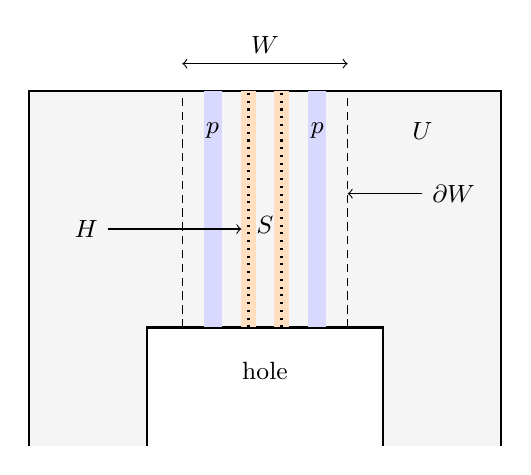
\begin{tikzpicture}[x=1cm,y=1cm,font=\small]
  \fill[gray!8] (-3,-1.5) rectangle (3,3);
  \fill[white] (-1.5,-1.5) rectangle (1.5,0);
  \draw[thick] (-3,-1.5)--(-3,3)--(3,3)--(3,-1.5);
  \draw[thick] (-1.5,-1.5)--(-1.5,0)--(1.5,0)--(1.5,-1.5);
  \fill[blue!15] (-.78,0) rectangle (-.55,3);
  \fill[blue!15] (.55,0) rectangle (.78,3);
  \fill[orange!25] (-.3,0) rectangle (-.12,3);
  \fill[orange!25] (.12,0) rectangle (.3,3);
  \draw[densely dashed] (-1.05,0)--(-1.05,3);
  \draw[densely dashed] (1.05,0)--(1.05,3);
  \draw[dotted,thick] (-.21,0)--(-.21,3);
  \draw[dotted,thick] (.21,0)--(.21,3);
  \node at (0,-.55) {hole};
  \node at (2,2.5) {\(U\)};
  \node at (0,1.3) {\(S\)};
  \node at (-.665,2.5) {\(p\)};
  \node at (.665,2.5) {\(p\)};
  \draw[->] (-2,1.25)--(-.3,1.25);
  \node[anchor=east] at (-2,1.25) {\(H\)};
  \draw[->] (2,1.7)--(1.05,1.7);
  \node[anchor=west] at (2,1.7) {\(\partial W\)};
  \draw[<->] (-1.05,3.35)--(1.05,3.35);
  \node[above] at (0,3.35) {\(W\)};
 \end{tikzpicture}
 \caption{A straight part of a strip \(S\) joining a hole to the
 outer free wall. Dotted lines indicate the interfaces cut to isolate
 \(S\). The pin region \(H\), shown along both interfaces, contains
 every endpoint of every lattice edge crossing either interface.
 The two
 guard bands \(p\) separate them from the artificial boundary of the
 wider patch \(W\). All bands have positive widths and positive
 intervening gaps. Parallel collars give the same separation at
 rectilinear turns. The bottom ends of the outer boundary and hole
 are omitted from the schematic.}
 \label{sectors:slit-figure}
\end{figure}


For prescribed absolute primary data \(u\) on \(p\), let
\[
 K^s(u)=\frac{Z_{\rm open}^s(u)}{Z_{\rm cut}^s(u)},
 \qquad d_0=K^0(0).
\]
Conditioning on the full guard separates the restored edges from
everything beyond \(W\), since no observation cell crosses a guard
division. Therefore \(K^s(u)\) is unchanged if we cut the edges
across \(\partial W\) and compute it using \(W\) alone.
The prescribed-data comparison of
Lemma~\ref{heights:cut-comparison} gives
\[
 \frac{Z_{\rm open}^s(u)}{Z_{\rm open}^0(0)}
 \le
 \frac{Z_{\rm cut}^s(u)}{Z_{\rm cut}^0(0)},
 \qquad\hbox{hence}\qquad 0<K^s(u)\le d_0.
\]

\emph{The loss inside the patch.}
Choose a union of positive-area boxes \(H\) containing all endpoints
of restored edges and positively separated from \(p\), in the cut
patch. Under its centered confined law,
\[
 1\ge \E_{{\rm cut}\,W,0}\frac{K^0(u)}{d_0}
 \ge e^{-D_{n,d}(H,p)}.
\]
To verify the lower bound, compare the restored partition sums with
guard data \(u\) and \(0\), then add the pin \(h_H=0\).
Precision comparison decreases their ratio. With \(H\) pinned,
restoration is a fixed scalar because all restored-edge endpoints
are fixed. Dividing by the corresponding cut-patch data ratio gives
the pointwise lower comparator
\[
 \frac{K^0(u)}{d_0}
 \ge
 \frac{\Pbb_{{\rm cut}\,W,0}(h_H=0\mid h_p=u)}
      {\Pbb_{{\rm cut}\,W,0}(h_H=0\mid h_p=0)}.
\]
Averaging and using Bayes' rule gives the displayed estimate.
Lemma~\ref{sectors:localization} shows that its lower bound tends
to one, in the order \(n\to\infty\), then \(d\downarrow0\).

Both versions of \(W\) have lifts, and the cuts remove only
zero-area interfaces. Lemma~\ref{sectors:single-lift} therefore
gives the same limit for their shifted-to-centered ratios.
It follows that
\begin{equation}
 \sum_u\frac{Z_{{\rm cut}\,W}^s(u)}{Z_{{\rm cut}\,W}^0}
           \left(1-\frac{K^s(u)}{d_0}\right)\longrightarrow0
 \quad(n\to\infty,\ \text{then }d\downarrow0).
 \tag{6}\label{eq:source-6}
\end{equation}
The arrow means that the iterated limsup is zero.
For clarity, the sum in Equation~\eqref{eq:source-6} is exactly
\[
 F_{{\rm cut}\,W}^s-
 F_{{\rm open}\,W}^s\,
       \E_{{\rm cut}\,W,0}\frac{K^0}{d_0}.
\]
This identity proves the assertion without any approximation of
conditional laws at individual microscopic values \(u\).

\emph{Passing from the patch to the whole domain.}
Let \(G\) be the current topology with the narrow strip cut, and
let \(G'\) be obtained by further cutting the edges across the
artificial boundary of \(W\). At prescribed guard data, precision
comparison gives
\[
 \frac{Z_G^s(u)}{Z_G^0(0_p)}
 \le \frac{Z_{G'}^s(u)}{Z_{G'}^0(0_p)}.
\]
Here \(0_p\) denotes prescribed zero guard data; a denominator without
a data argument sums over those data. Thus
\begin{equation}
 \frac{Z_G^s(u)}{Z_G^0}
 \le
 \frac{\Pbb_{G,0}(h_p=0)}{\Pbb_{G',0}(h_p=0)}
 \frac{Z_{G'}^s(u)}{Z_{G'}^0}.
 \label{sectors:global-data-bound}
\end{equation}
This change of normalization has a controlled cost.
Let \(R(u)\) be the centered restoration factor from \(G'\) to \(G\)
at guard data \(u\). Directly summing partition functions gives
\[
 \frac{\Pbb_{G,0}(h_p=0)}{\Pbb_{G',0}(h_p=0)}
 =\frac{R(0)}{\E_{G',0}R}.
\]
Choose a union of boxes \(H'\) containing the endpoints of all
edges across the artificial boundary of \(W\), separated from \(p\).
The preceding centered restoration comparison, now with \(H'\),
implies
\[
 \frac{\E_{G',0}R}{R(0)}
 \ge e^{-D_{n,d}^{G'}(H',p)}.
\]
Lemma~\ref{sectors:localization} makes this interaction tend to zero.
All observation cells remain within their components after the cut,
and control their constants, so its hypotheses hold for \(G'\).

Multiply Equation~\eqref{sectors:global-data-bound} by the
nonnegative quantity \(1-K^s(u)/d_0\) and sum.
On \(G'\), the part outside \(W\) factors off as a
shifted-to-centered confined ratio, at most one by
Lemma~\ref{heights:finite-comparisons}.
The resulting global loss is therefore at most
\(e^{D_{n,d}^{G'}(H',p)}\) times the patch loss in
Equation~\eqref{eq:source-6}; it tends to zero.
The same conclusion applies to the centered loss.

To finish, define these two losses on the current cut graph by
\[
 L_s=\sum_u\frac{Z_{\rm cut}^s(u)}{Z_{\rm cut}^0}
                 \left(1-\frac{K^s(u)}{d_0}\right),
 \qquad
 L_0=\E_{{\rm cut},0}\left(1-\frac{K^0}{d_0}\right).
\]
Summing the restored numerator and denominator gives the exact identity
\begin{equation}
 F_{\rm open}^s=\frac{F_{\rm cut}^s-L_s}{1-L_0}.
 \label{sectors:restoration-identity}
\end{equation}
Since \(L_s,L_0\) tend to zero in the prescribed order and
\(F_{\rm cut}^s\le1\), a strip deletion changes the confined ratio
by a quantity tending to zero. There are only finitely many strips.
After all deletions, Lemma~\ref{sectors:single-lift} identifies the
product ratio with the right side of Equation~\eqref{eq:source-5}.
The energies add over the pieces to \(\int_U|dv|^2\).
Restoring the strips proves the proposition. The raw factors \(d_0\)
cancel in Equation~\eqref{sectors:restoration-identity}; no bound on
their size is needed.
\end{proof}

\begin{proof}[Completion of Theorem~\ref{sectors:positive-radius}]
For every smooth \(g\) near \(\overline U\), combine
Equation~\eqref{sectors:confinement-lower} with
Proposition~\ref{sectors:weighted} to obtain
\[
 \liminf_{n\to\infty}F_{U,n}^s
 \ge \exp\left\{-\frac1{2a}\int_U|dv_0+dg|^2\right\}.
\]
Restrictions of smooth functions from a neighborhood are dense in
\(H^1(U)\), since \(U\) is Lipschitz. Let their energies approach
\(\mathcal M(U)\). This proves the lower bound in
Equation~\eqref{eq:source-3}, and the earlier upper bound proves the
limit. Every use of a height or pin theorem was at fixed geometry
and fixed \(d\); all subsequent limits were taken afterwards.
\end{proof}
